\section{Theorie}

Die Beugung ist ein Phänomen, welches auftritt, sobald Lichtwellen auf ein Hindernis treffen, dessen Spaltbreite klein genug ist. Diese muss klein im Vergleich zur Strahlenbreite des Lichtstrahls sein. Das kann mit dem Huygenschen Prinzip erklärt werden. Demnach ist jeder Punkt der Wellenfront eine Quelle einer neuen Welle. Das bedeutet, dass aus dem Teil der Wellenfront, welche durch den Spalt durchkommt, weitere kugelförmige Wellen austreten. Folglich bildet sich ein Intensitätsmuster am Schirm mit Maxima und Minima, wohingegen das globale Maxima jenes nullter Ordnung ist. Die Höhen der anderen Maxima nehmen in der Theorie stets ab.\\
Für die Berechnung der Intensität des abgebeugten Lichts gibt es zwei Näherungen. Zunächst gibt es die Fresnelsche Näherung, welche unter der Gegebenheit, dass Lichtquelle und jeglicher Beobachtungspunkt auf dem Schirm eine endliche Distanz zueinander haben, angenommen werden kann. Dabei haben die Lichtstrahlen einen divergierenden Verlauf.\\
Eine andere Näherung, die Fraunhofersche Näherung, ist die Annahme, dass die Distanz zwischen Lichtquelle und Schirm unendlich groß ist. Dementsprechend divergieren die Lichtstrahlen so wenig voneinander, dass diese als parallel angenommen werden können.\\
Mithilfe vom letzteren kann die Beugung am Spalt durch folgende Skizze beschrieben werden:

\begin{figure}
    \centering
    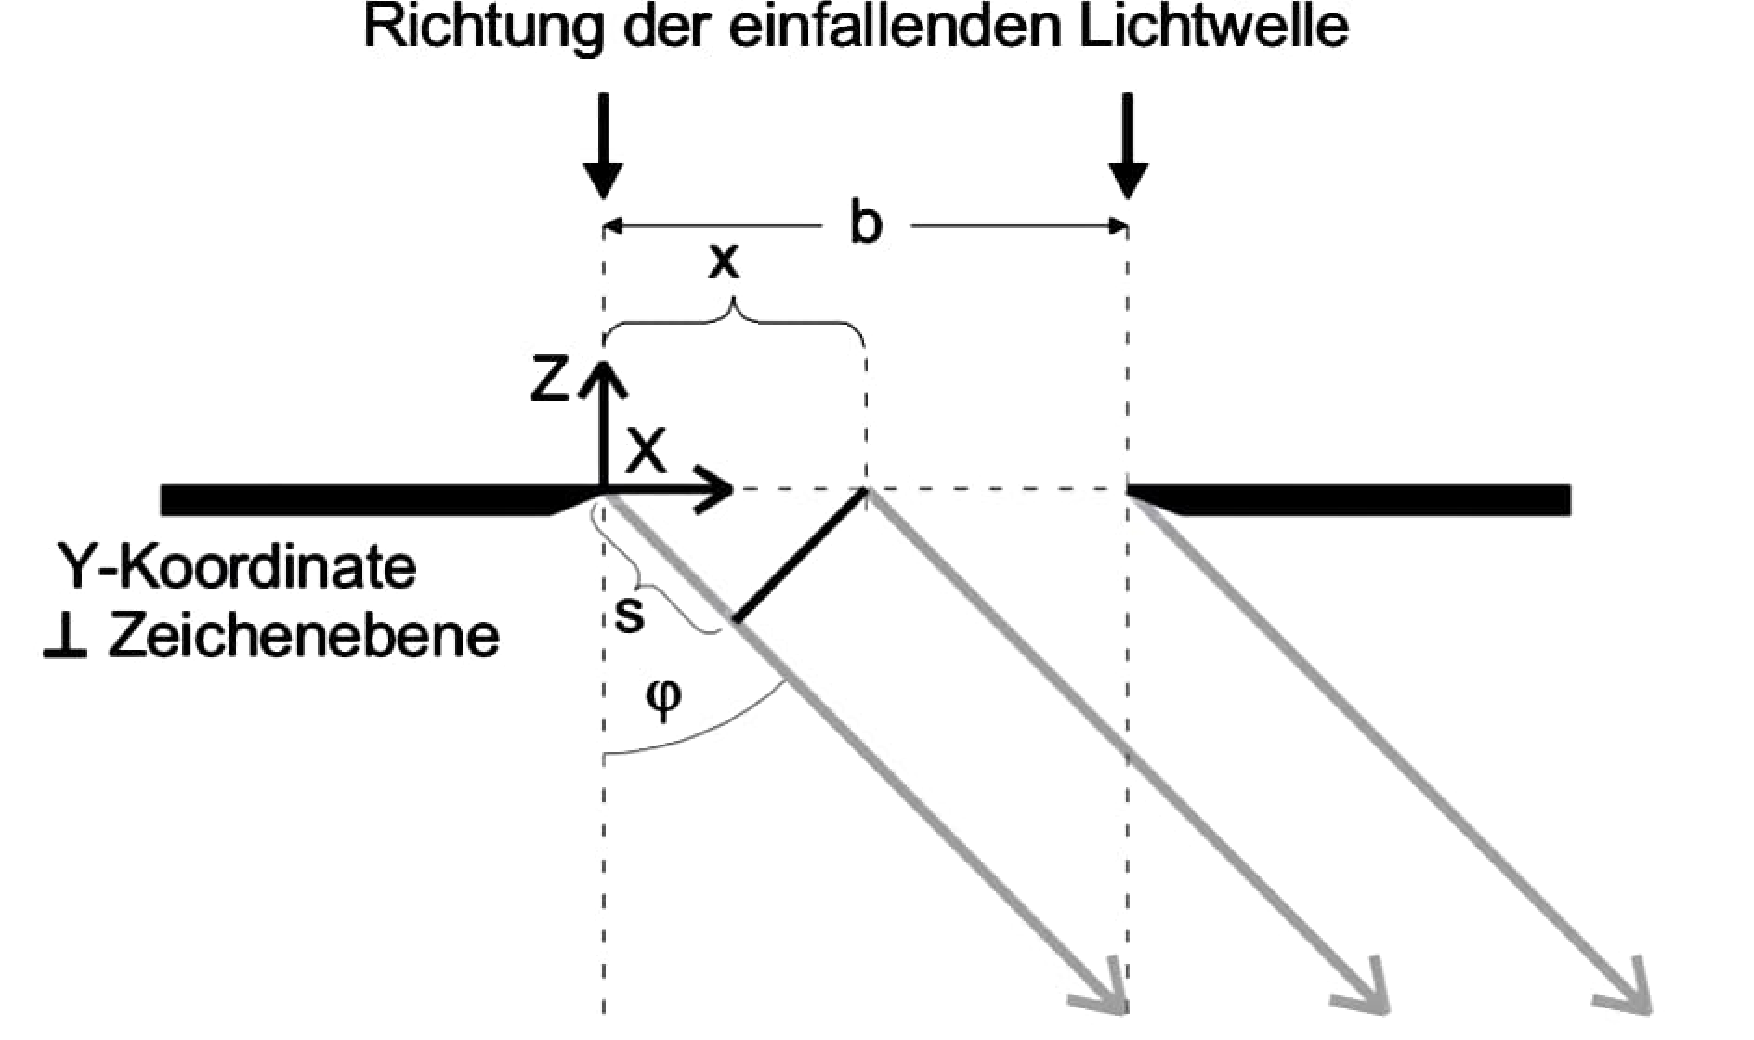
\includegraphics[scale=0.5]{content/Einzelspalt.pdf}
    \caption{Hier zu sehen ist die graphische Darstellung der Beugung am Einzelspalt.}
    \label{fig:one}
\end{figure}

\begin{figure}
    \centering
    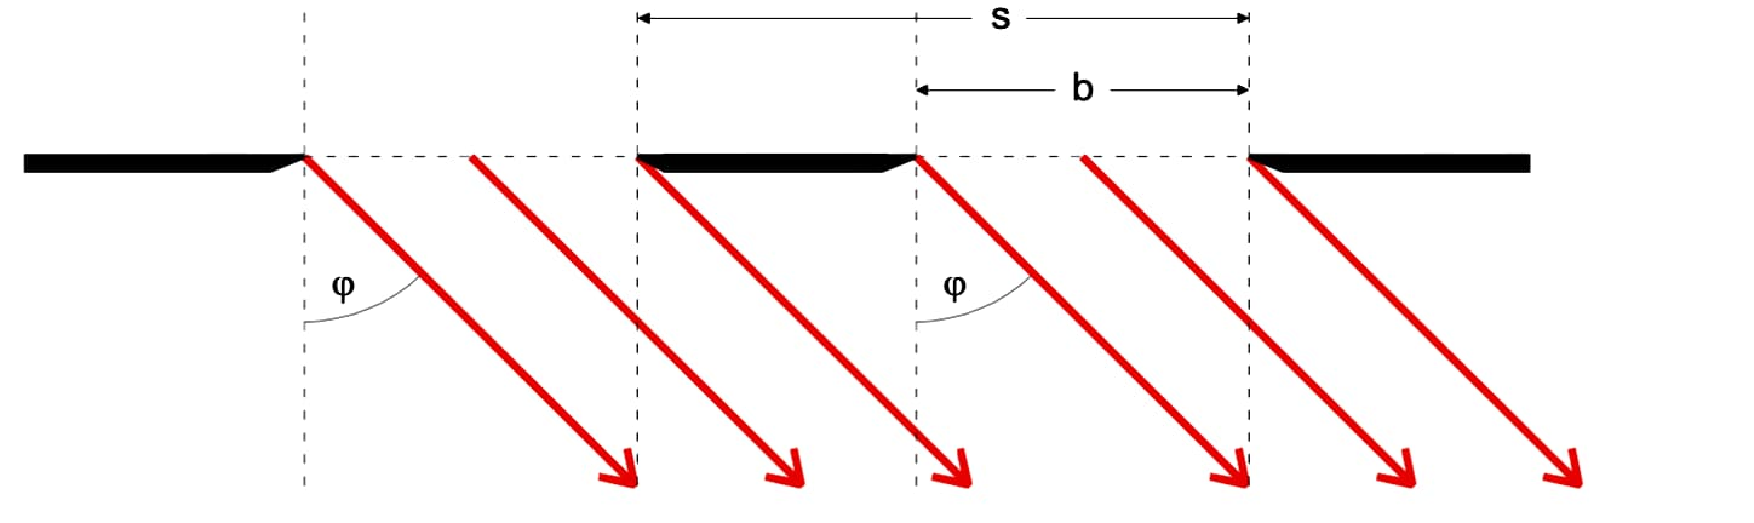
\includegraphics[scale=0.5]{content/Doppelspalt.pdf}
    \caption{Hier zu sehen ist die graphische Darstellung der Beugung am Doppelspalt.}
    \label{fig:single}
\end{figure}

Dabei entstehen zwischen den Lichtstrahlen zusätzlich Wegunterschiede \(\delta\), die durch 

\begin{equation}
    \delta = \frac{2\pi x \sin(\phi)}{\lambda}
\end{equation}

Dabei ergibt sich für die Amplitude \(B\) nach Integration 

\begin{equation}
    B(z,t,\phi) = A_0 e^{i(\omega t - \frac{2\pi z}{\lambda})} e^{\frac{\pi ib\sin(\phi)}{\lambda}} \frac{\lambda}{\pi \sin(\phi)} \sin(\frac{\pi b\sin(\phi)}{\lambda}).
    \label{eq:es}
\end{equation}

Dabei ist \(\omega\) die Kreisfrequenz, des Lichts, \(\lambda\) die Wellenlänge, \(b\) die Spaltenbreite, \(z\) der Abstand zum Schirm bzw. dem Beobachtungspunkt darauf und \(\phi\) ist in der Skizzierung zu sehen.\\
\(B\) hat unendlich viele Null- und Extremstellen, wobei sie für wachsendes \(\phi\) gegen Null konvergiert.\\
Die Intensität \(I\) ergibt sich mit

\begin{equation}
    \eta = \frac{\pi b \sin(\phi)}{\lambda}
\end{equation}

und \(I\) \(\propto\) \(B^2\) zu

\begin{equation}
    I \propto A_0^2 b^2 \frac{\lambda^2}{\pi^2 b^2 \sin(\phi)^2} \sin^2(\frac{\pi b \sin(\phi)}{\lambda}).
\end{equation}

Speziell für die Beugung am Doppelspalt ergibt sich obige Gleichung zu

\begin{equation}
    I \propto 4 \cos^2(\frac{\pi s \sin(\phi)}{\lambda}) \frac{\lambda^2}{\pi^2 b^2 \sin(\phi)^2} \sin^2(\frac{\pi b \sin(\phi)}{\lambda}).
\end{equation}

Zum Schluss ist noch die Fourier-Transformation zu behandeln. Diese (komplex) ist definiert als

\begin{equation}
    g(y) = {\int_{-\infty}}^{+\infty} B(x) e^{ixy} dx
\end{equation}

und woraus folgt, dass 

\begin{equation}
    g(y) = \frac{2A_0}{y} e^{\frac{iyb}{2}}\sin(\frac{yb}{2})
\end{equation}

mit 

\begin{equation}
    y = \frac{2\pi\sin(\phi)}{\lambda}.
\end{equation}

Hier wird das Huygenssche Prinzip ersichtlich, da der zweite Faktor, also die E-Funktion, die Phasendifferenz der von \(x\) ausgehenden Kugelwelle beschreibt. Das Integral, also praktisch eine Aufsummation von allen Erregungszentren im Integrationsbereich, berücksichtigt auch die jewiligen Phasen. Die Fourier-Transformation kann zudem auch noch umgekehrt und auf mehreren Dimensionen erweitert werden, was bei Kugelwellen ihre Praktizierbarkeit findet.

\cite{sample}
\label{sec:Theorie}